\documentclass[conference]{IEEE}
\IEEEoverridecommandlockouts
\usepackage{cite}
\usepackage{amsmath,amssymb,amsfonts}
\usepackage{algorithmic}
\usepackage{graphicx}
\usepackage{textcomp}
\usepackage{xcolor}
\usepackage{parskip}
\usepackage{setspace}
\usepackage{hyperref}
\usepackage{pgfplots}
\pgfplotsset{compat=1.17}
\usepackage{tikz}
\usetikzlibrary{shapes.geometric,arrows.meta,positioning,calc,fit,backgrounds}

\setstretch{1.0}

\def\BibTeX{{\rm B\kern-.05em{\sc i\kern-.025em b}\kern-.08em
    T\kern-.1667em\lower.7ex\hbox{E}\kern-.125emX}}

\newcommand*{\affaddr}[1]{#1}
\newcommand*{\affmark}[1][*]{\textsuperscript{#1}}

\begin{document}

\title{AI-Based Railway Track Defect Detection in India:\\False Negatives, Safety Assurance and Human Accountability}

\author{
    Jivetesh\affmark[*], Kathir Kalidass B\affmark[*], Dhinesh Babu C M\affmark[*], Paril T\affmark[*]\\[0.5em]
    \affaddr{\affmark[*]College of Engineering, Guindy (CEG),\\Anna University, Chennai -- 600025, India}
}

\maketitle

% ============================================================
\begin{abstract}
Railway track safety constitutes a domain where undetected surface defects can precipitate catastrophic derailments with devastating human and economic consequences. Artificial intelligence (AI) systems based on computer vision have shown promising results in automating visual inspection of railway tracks, yet their deployment in safety-critical environments raises fundamental Responsible AI (RAI) concerns regarding reliability under field conditions, transparency of decisions, and accountability for outcomes. This case study investigates AI-based railway track defect detection through the lens of Responsible AI, with specific reference to the Indian railway context. We examine five critical dimensions: false negative rates and their safety consequences, model robustness under adverse environmental conditions prevalent in Indian railway divisions, explainability of AI decisions for inspector verification, human accountability frameworks aligned with existing governance structures, and safety assurance protocols for pre-deployment validation. Through a systematic review of peer-reviewed research published between 2022 and 2025, analysis of Indian Railways technical standards, and a reproducible experimental implementation on a publicly available rail defect dataset, we demonstrate that high overall accuracy alone is insufficient for safety-critical deployment. Our results reveal that a CNN achieving 93.2\% accuracy under ideal conditions exhibits a false negative rate of 8.5\%, which escalates to 22.7\% under combined adverse environmental conditions -- a 2.7-fold increase in missed defects. We propose a human-in-the-loop framework that preserves qualified inspector oversight, mandates uncertainty escalation, and maintains established railway safety procedures as the authoritative decision-making layer. The key contribution is a structured RAI analysis connecting technical model performance metrics to governance requirements for safe AI deployment in Indian railway infrastructure.
\end{abstract}

% ============================================================
\begin{IEEEkeywords}
Responsible AI, Railway Infrastructure, Computer Vision, Safety-Critical Systems, False Negative Rate, Explainability, Human Accountability, Defect Detection, Indian Railways, Grad-CAM
\end{IEEEkeywords}

% ============================================================
\section{Introduction}
% ============================================================

Railway transportation constitutes the backbone of India's transportation infrastructure, with Indian Railways operating over 68,000 route-kilometres and transporting more than 23 million passengers daily across 13,000 passenger trains and 9,000 freight trains \cite{pib2017}. The safety and reliability of this vast network depend critically upon the integrity of railway tracks, where undetected surface defects -- including transverse cracks, head checks, squats, and shelling -- can precipitate catastrophic derailments with severe human and economic consequences \cite{khajeh2025}. The cascading impact of a single derailment extends beyond immediate casualties to include network disruption, freight delays, and erosion of public confidence in railway safety.

Traditional inspection methodologies, encompassing Track Recording Cars (TRC), Oscillation Monitoring Systems (OMS), ultrasonic testing, and manual patrolling, remain resource-intensive and cannot deliver continuous, comprehensive coverage across the entire network \cite{rdso2020}. The sheer scale of the network -- combined with challenging geographic and climatic conditions -- creates a compelling case for augmenting existing inspection methods with intelligent automation. However, the integration of AI into safety-critical railway operations demands rigorous evaluation through the Responsible AI framework, which mandates that AI systems be safe, explainable, fair, and subject to meaningful human oversight.

This case study investigates AI-based railway track defect detection through the lens of Responsible AI, with particular emphasis on the Indian railway context. Our investigation addresses the following research questions:

\begin{enumerate}
    \item \textbf{False Negatives:} Can a model achieving high overall accuracy still classify defective rail sections as normal, and what are the safety consequences of such misclassifications?
    \item \textbf{Robustness:} How does detection performance vary under poor lighting, dirt, rust, shadows, and diverse track conditions representative of Indian railway divisions?
    \item \textbf{Explainability:} Can railway inspectors understand why a model flagged or failed to flag a suspected defect, and does the explanation support effective verification?
    \item \textbf{Human Accountability:} Who verifies AI alerts, authorises maintenance actions, and bears responsibility for safety decisions?
    \item \textbf{Safety Assurance:} How should uncertainty, model errors, and system failures be managed before, during, and after deployment?
\end{enumerate}

The central thesis of this study is that AI should \textit{support} railway inspectors rather than \textit{replace} mandatory inspection procedures and engineering judgement. A camera-based AI system, regardless of its reported accuracy, cannot detect internal rail flaws that require ultrasonic or other non-destructive testing methods \cite{rdso2020}. Its legitimate role is to function as a decision-support tool that identifies visible surface defects efficiently and flags them for qualified human review.

The remainder of this paper is structured as follows: Section~\ref{sec:background} provides domain background and the Indian railway context. Section~\ref{sec:related} reviews related research on AI-based defect detection. Section~\ref{sec:rai} applies Responsible AI principles to railway inspection. Section~\ref{sec:technical} presents the technical problem formulation and existing methods. Section~\ref{sec:explainability} discusses explainability approaches. Section~\ref{sec:safety} addresses safety, security, and privacy considerations. Section~\ref{sec:implementation} describes the dataset, model, and experimental analysis. Section~\ref{sec:framework} proposes a human-in-the-loop framework. Section~\ref{sec:conclusion} presents conclusions and recommendations.

% ============================================================
\section{Background and Indian Railway Context}
\label{sec:background}
% ============================================================

\subsection{Railway Track Safety in India}

Indian Railways operates under challenging geographic and climatic conditions that accelerate rail defect formation. Rail defects develop progressively: surface cracks initiate from rolling contact fatigue accelerated by high axle loads and traffic density; corrosion intensifies in coastal and high-humidity regions; and thermal stresses cause fractures in regions with temperature extremes. The Research Designs and Standards Organisation (RDSO) prescribes ultrasonic testing standards in Document No.\ T-53 (Revised 2020), specifying defect-detection reliability requirements and operator competency criteria \cite{rdso2020}.

Current inspection infrastructure includes: Track Recording Cars (TRC) for track geometry measurement, Oscillation Monitoring Systems (OMS) for indirect track condition assessment, Ultrasonic Testing using Single Rail Testers (SRT) and Double Rail Testers (DRT), and foot and motorised patrolling by section engineers and trackmen \cite{pib2017}. These methods are effective but labour-intensive and deployed at discrete intervals. An AI-based visual inspection system should extend the reach of existing methods, not duplicate or replace them.

Current inspection infrastructure deployed by Indian Railways includes:

\begin{itemize}
    \item \textbf{Track Recording Cars (TRC):} Automated vehicles equipped with sensors measuring track geometry at speeds up to 100 km/h, requiring scheduled deployment \cite{pib2017}.
    \item \textbf{Ultrasonic Testing:} Single Rail Testers (SRT) and Double Rail Testers (DRT) detect internal rail defects through non-destructive testing. Self-Propelled Ultrasonic Rail Testing (SPURT) cars were under planned procurement \cite{pib2017}.
    \item \textbf{Foot and Motorised Patrolling:} Section engineers and trackmen conduct visual inspections, supplemented by periodic monitoring.
    \item \textbf{Distributed Optical-Fibre Sensing:} Under trial for rail-fracture detection, representing a different sensing paradigm from camera-based approaches.
\end{itemize}

These methods are operationally effective but labour-intensive, deployed at discrete intervals, and limited by human visual acuity under field conditions. An AI-based visual inspection system using cameras mounted on inspection vehicles could complement existing methods by providing high-frequency, high-resolution monitoring of rail surface conditions \cite{pib2017}. The key word is \textit{complement}: the AI system should extend the reach of existing inspection, not duplicate or replace it.

\subsection{Limitations of Visual Inspection}

A critical distinction must be maintained throughout this analysis: \textbf{visual inspection detects surface defects only}. Internal flaws, including hydrogen-induced cracks, gauge corner cracking below the surface, weld defects, and internal rail fractures, require ultrasonic testing or other appropriate non-destructive methods \cite{rdso2020}. Presenting an AI vision system as a substitute for these established safety procedures would be both technically unsound and ethically unacceptable in a safety-critical domain.

Surface defects potentially detectable through visual inspection include transverse cracks, longitudinal cracks, squats, shelling, head wear, and fastening abnormalities. The severity spectrum ranges from minor surface scratches posing minimal operational risk to full-depth transverse cracks capable of causing immediate derailment under load. The RDSO specification for ultrasonic testing (T-53, 2020) requires verified defect-detection reliability, with repeated testing against known defects and artificial reference standards \cite{rdso2020}. While this standard does not directly certify AI image classifiers, it establishes the safety-assurance philosophy that any inspection system must approach: verified reliability against known defect types, with qualified operators maintaining documented competency.

% ============================================================
\section{Related Work}
\label{sec:related}
% ============================================================

\subsection{Deep Learning Approaches for Railway Defect Detection}

The application of deep learning to railway defect detection has advanced rapidly. Khajehdezfuly et al.\ \cite{khajeh2025} conducted a systematic review of 567 studies (2002--2025), revealing that 88\% employ on-board data acquisition with image and video as the primary input modalities. The review identifies rails and fastening systems as the most studied components, reflecting their critical safety role.

Alif et al.\ \cite{alif2026} provide a comprehensive survey of computer vision applications in railway engineering, noting that multi-sensor fusion -- combining cameras with LiDAR, infrared sensors, and ultrasonic transducers -- offers the most robust inspection approach. Single-sensor vision systems remain vulnerable to environmental factors including rain, fog, dust, and lighting variation, which significantly degrade detection performance \cite{alif2026}.

\subsection{YOLO-Based Detection Methods}

YOLO architectures have gained prominence for railway crack detection due to real-time inference capability. A comparative study at IEEE IEMCON 2024 evaluated YOLOv5 and YOLOv9 for automated crack detection, reporting F1-scores of 0.92 and 0.91 respectively alongside explainable AI visualisation \cite{yolo2024}. An F1-score of 0.92 implies approximately one in ten defective sections is missed or falsely flagged -- unacceptable for railway safety without human verification, motivating our focus on false negative rate as the primary metric.

\subsection{Research Gaps}

Kumar and Harsha \cite{kumar2025} identify four critical gaps in machine vision-based railway defect detection: (1) limited Indian railway datasets capturing local defect patterns and environmental conditions; (2) insufficient robustness evaluation under realistic field conditions; (3) minimal attention to explainability for inspector trust; and (4) absence of governance frameworks for deployment accountability. The IEEE Access systematic review \cite{ieee2025} similarly identifies explainability and safety standard compliance as unresolved challenges for operational deployment.

% ============================================================
\section{Responsible AI Principles for Railway Inspection}
\label{sec:rai}
% ============================================================

Deploying AI systems in railway track inspection requires the application of Responsible AI principles tailored to the specific requirements of a safety-critical transportation domain. Figure~\ref{fig:taxonomy} presents the six core RAI principles as an interconnected framework, and Table~\ref{tab:rai_principles} summarises each principle with its specific application to railway inspection and the consequences of neglect.

\begin{figure}[ht]
  \centering
  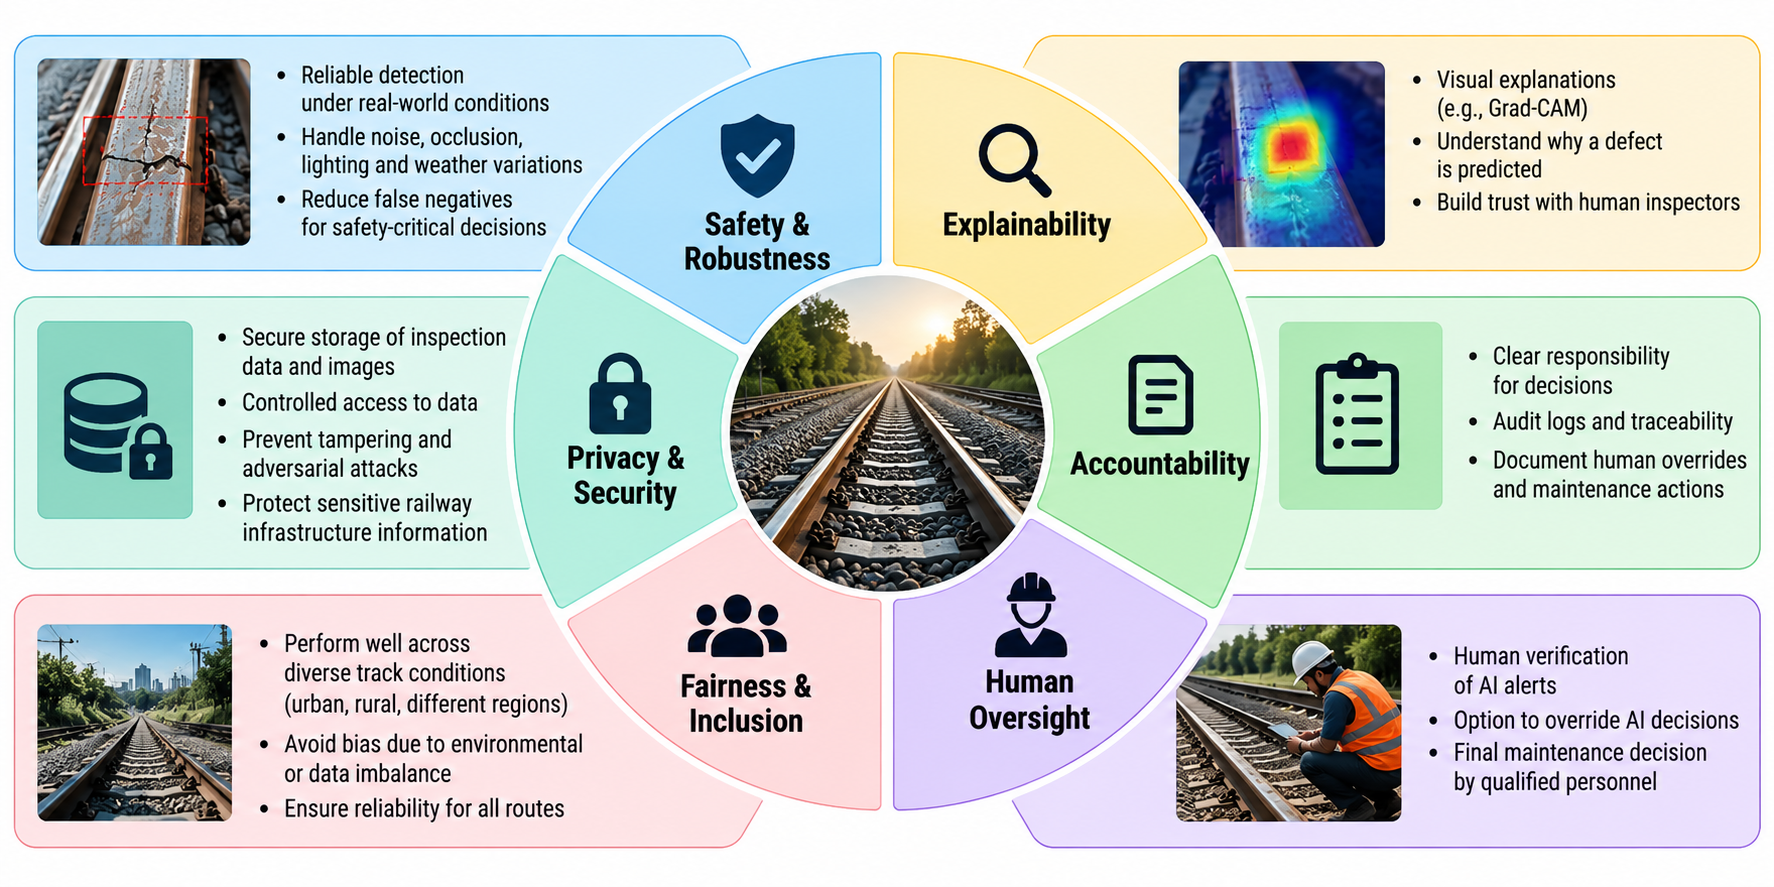
\includegraphics[width=\linewidth]{fig_taxonomy.png}
  \caption{Responsible AI principles taxonomy for railway track defect detection, showing the six core principles and their interrelationships in a safety-critical deployment context.}
  \label{fig:taxonomy}
\end{figure}

\begin{table}[ht]
\caption{Responsible AI Principles for Railway Track Defect Detection}
\label{tab:rai_principles}
\centering
\renewcommand{\arraystretch}{1.2}
\begin{tabular}{|p{2.4cm}|p{5.4cm}|}
\hline
\bfseries Principle & \bfseries Application \& Risk if Neglected \\
\hline
Safety \& Robustness & Detection must perform reliably across lighting, weather, surface conditions, and track environments. \newline \textit{Risk:} Missed defects leading to derailment \\
\hline
Explainability & Inspectors must understand which image regions influenced a classification decision. \newline \textit{Risk:} Unexplained alerts ignored or mistrusted by field personnel \\
\hline
Accountability & Clear ownership of alert verification, escalation procedures, and maintenance authorisation. \newline \textit{Risk:} Safety failures with no identifiable responsible party \\
\hline
Human Oversight & Qualified personnel must review AI outputs before any consequential maintenance decision. \newline \textit{Risk:} Autonomous incorrect decisions with no override mechanism \\
\hline
Fairness \& Inclusion & Consistent detection performance across defect categories, track sections, and geographic regions. \newline \textit{Risk:} Undetected defects in under-represented scenarios \\
\hline
Privacy \& Security & Protection of inspection footage, operational records, and system access controls. \newline \textit{Risk:} Unauthorised data access or adversarial model manipulation \\
\hline
\end{tabular}
\end{table}

These principles are not independent. A failure in explainability undermines human oversight; weak accountability erodes safety assurance; inadequate robustness testing compromises fairness across deployment sites. The following subsections examine each principle in the railway inspection context.

\subsection{Safety and Robustness}

The paramount RAI principle for railway inspection is safety. A defect detection system must maintain adequate performance across the full range of operational conditions encountered in Indian railway divisions. As demonstrated in our experimental analysis (Section~\ref{sec:implementation}), accuracy measured under ideal laboratory conditions does not reliably predict field performance. Rain accumulation on camera lenses, mud splashes on rail surfaces, variable sunlight angles, shadow patterns from vegetation, and seasonal surface contamination all affect image quality and, consequently, detection reliability \cite{ieee2025}.

Safety in this context means more than achieving a target accuracy metric. It means the system behaves predictably and reliably across the full operational envelope, degrades gracefully when conditions deteriorate, and communicates its uncertainty transparently to human operators. A model that produces high-confidence incorrect classifications under adverse conditions is more dangerous than one that expresses low confidence and escalates to human review.

\subsection{Explainability}

Railway inspectors require meaningful explanations to trust AI recommendations and perform effective independent verification. A heatmap highlighting the specific image region that influenced a classification decision enables the inspector to cross-reference the AI output with their own visual assessment. Without explainability, an AI system becomes an opaque black box that field personnel are likely to override indiscriminately -- negating its practical value while creating liability exposure when it produces correct alerts \cite{kumar2025}.

Explainability also serves a model-development function. By examining Grad-CAM visualisations during training and validation, researchers can identify whether the model has learned genuine defect features or spurious correlations -- such as attending to the ballast texture, rail fasteners, or shadow patterns rather than the defect itself.

\subsection{Human Accountability}

The Indian Railways inspection hierarchy assigns clear responsibilities: section engineers verify track conditions at the ground level, divisional engineers approve maintenance programmes, and the RDSO sets technical standards and certification requirements \cite{rdso2020}. An AI system must integrate within this existing governance structure rather than establishing parallel decision-making authority. The individual who reviews an AI-generated alert and authorises maintenance action must be identifiable, appropriately trained, and empowered to override the system's recommendation \cite{pib2017}.

The RDSO ultrasonic testing specification T-53 (2020) requires that operators hold valid competency certificates and that inspection activities be documented for traceability \cite{rdso2020}. These principles translate directly to AI-assisted inspection: the human reviewer of AI alerts should possess appropriate railway engineering qualifications, and all AI-assisted inspection decisions should be recorded in a tamper-evident audit trail.

\subsection{Human Oversight}

The human-in-the-loop principle is not merely an architectural preference but a safety requirement for high-consequence domains. Inspectors must retain the ability to override AI classifications when their professional engineering judgement disagrees with the model output, escalate uncertain or conflicting results through established channels, initiate manual inspection procedures regardless of AI output, and document their decisions for audit trails and continuous model improvement. This principle aligns with the RDSO practice of confirming over-reported defects through additional testing or alternative methods \cite{rdso2020} -- no single source of evidence, AI or otherwise, should be treated as conclusive without human confirmation.

\subsection{Fairness and Inclusion}

Railway tracks in India traverse diverse geographic and climatic regions: coastal routes with salt corrosion, desert routes with sand abrasion, high-altitude routes with extreme temperature variation, and high-traffic corridors with accelerated wear patterns. A model trained predominantly on data from one region may fail to generalise effectively to others. Ensuring equitable detection performance across defect categories and track environments requires representative training data and stratified evaluation across operational divisions.

This principle has both technical and social dimensions. Technically, it requires evaluating model performance separately for each defect type and environmental condition, identifying where performance degrades, and addressing gaps through targeted data collection or model adaptation. Socially, it requires that inspection quality not vary systematically based on the geographic or economic characteristics of the railway division -- a concern if AI systems are deployed unevenly across the network.

\subsection{Privacy and Security}

Inspection footage contains operational data about railway infrastructure, potential security-sensitive details about track geometry, and geolocation data. System security must protect against unauthorised access to inspection records, adversarial manipulation of input images, and tampering with model parameters. Access controls and comprehensive audit logging are essential components of a responsible deployment architecture.

The IEEE Access systematic review \cite{ieee2025} identifies adversarial robustness as a key unresolved challenge in railway AI research. Adversarial perturbations -- carefully crafted modifications to input images -- can cause deep learning models to misclassify defects. In a deployment context, such attacks could be deliberate acts of sabotage or inadvertent image corruption during transmission. Defensive strategies include input validation pipelines, ensemble model architectures, and continuous monitoring for distribution shifts in incoming inspection data.

% ============================================================
\section{Technical Problem and Existing Methods}
\label{sec:technical}
% ============================================================

\subsection{Problem Formulation}

The railway track defect detection task can be formalised as a binary classification problem: given an image $I$ of a railway rail surface, the model $f$ must predict a class label $y \in \{0, 1\}$, where $y = 1$ indicates the presence of a surface defect and $y = 0$ indicates a normal surface. The model outputs a confidence score $p = f(I) \in [0, 1]$, where $p$ represents the estimated probability of defect presence. A decision threshold $\tau$ determines the classification boundary: the image is classified as defective if $p \geq \tau$, and normal otherwise.

In safety-critical railway applications, the cost of a false negative (classifying a defective rail as normal) far exceeds the cost of a false positive (classifying a normal rail as defective). A false negative may result in an undetected defect progressing to catastrophic failure under repeated train loading, while a false positive merely triggers an additional inspection that confirms the rail's integrity. This asymmetric cost structure is formalised in the weighted loss function:

\begin{equation}
\mathcal{L} = \frac{1}{N} \sum_{i=1}^{N} \left[ w_{FN} \cdot \mathbb{I}(y_i=1, \hat{y}_i=0) + w_{FP} \cdot \mathbb{I}(y_i=0, \hat{y}_i=1) \right]
\end{equation}

where $w_{FN} \gg w_{FP}$ reflects the higher cost of false negatives, and $\mathbb{I}(\cdot)$ is the indicator function. For railway deployment, we propose $w_{FN} = 10$ and $w_{FP} = 1$, reflecting that a missed defect is at least an order of magnitude more costly than an unnecessary inspection.

\subsection{Existing AI Methods}

Convolutional neural networks (CNNs) have become the dominant architecture for railway defect detection. Wang et al.\ \cite{wang2022} proposed a deep learning approach using CNNs for surface defect classification on the NEU surface defect dataset, demonstrating effective classification of defect types including cracks, patches, and inclusions. However, the study noted significant performance degradation under varying illumination conditions and when defect severity is low -- precisely the conditions where false negatives are most dangerous.

ResNet architectures have been applied to railway defect detection with strong results, leveraging residual connections to enable training of deeper networks that capture hierarchical defect features \cite{yolo2024}. EfficientNet scaling strategies have been explored to balance model accuracy with computational efficiency for deployment on resource-constrained inspection vehicles.

Vision Transformers (ViT) represent a more recent approach, applying self-attention mechanisms to capture long-range dependencies in rail surface images. While ViTs show promise for complex defect patterns, they require larger training datasets and greater computational resources than CNNs, presenting deployment challenges in bandwidth-constrained railway environments \cite{alif2026}.

\subsection{Multi-Sensor Fusion}

The systematic review by Khajehdezfuly et al.\ \cite{khajeh2025} identifies multi-sensor fusion as a key research opportunity. Railway inspection data sources include image, video, acoustic, acceleration, ultrasonic, and satellite remote-sensing data. Each modality captures complementary aspects of rail condition: cameras detect visible surface defects, acoustic sensors identify internal cracks through sound propagation analysis, and ultrasonic testing remains the gold standard for internal flaw detection. A comprehensive inspection system should integrate these modalities while maintaining the distinct roles and reliability levels of each method. No single sensor can provide complete assurance of rail integrity.

% ============================================================
\section{Explainability and Interpretability}
\label{sec:explainability}
% ============================================================

\subsection{The Need for Explainability in Safety-Critical AI}

Explainability in railway defect detection serves two distinct purposes: \textit{model debugging} during the development phase and \textit{operational transparency} during field deployment. During development, explainability tools help researchers identify whether a model has learned genuine defect features or spurious correlations in the training data. During deployment, explainability enables inspectors to verify that the model's attention aligns with their own assessment, building the trust necessary for practical adoption.

The systematic review by Kumar and Harsha \cite{kumar2025} identifies explainability as one of the four critical research gaps in railway machine vision inspection. Field inspectors who cannot understand why an AI system flagged a particular region are unlikely to rely on its outputs, reducing the system's practical value despite high benchmark accuracy.

\subsection{Grad-CAM Methodology}

Gradient-weighted Class Activation Mapping (Grad-CAM), introduced by Selvaraju et al.\ \cite{selvaraju2017}, provides a visual explanation by highlighting the regions of an input image that most influenced the model's classification decision. For a crack detection CNN, a meaningful Grad-CAM heatmap should concentrate on the rail surface region containing the defect. When the heatmap highlights irrelevant regions -- such as the ballast, adjacent rails, or background scenery -- the explanation reveals that the model is attending to spurious correlations rather than genuine defect features.

The Grad-CAM computation proceeds as follows. Given a CNN with convolutional feature maps $A^k$ and a target class $c$, the gradient of the class score $y^c$ with respect to the feature maps is computed:

\begin{equation}
\frac{\partial y^c}{\partial A^k_{ij}}
\end{equation}

These gradients are global-average-pooled over the spatial dimensions to obtain neuron importance weights:

\begin{equation}
\alpha_k^c = \frac{1}{Z} \sum_i \sum_j \frac{\partial y^c}{\partial A^k_{ij}}
\end{equation}

where $Z$ is the number of pixels in each feature map. The weighted linear combination of feature maps produces the final heatmap:

\begin{equation}
L^c = \text{ReLU}\left(\sum_k \alpha_k^c A^k\right)
\end{equation}

The resulting heatmap $L^c$ is upsampled to the input image dimensions and overlaid as a colour-coded transparency, providing an intuitive visual explanation of the model's decision.

\subsection{Limitations of Explainability}

It is essential to recognise that an explanation does not constitute proof of correctness. Grad-CAM visualises \textit{where} the model directed its attention, not \textit{whether} it correctly identified a defect. A model can produce a plausible heatmap over a region containing no actual defect, or it can attend to the correct region but misclassify the severity or type of defect. Explainability increases inspector trust and aids model debugging, but it does not replace independent verification and established inspection procedures.

% ============================================================
\section{Safety, Security, and Privacy}
\label{sec:safety}
% ============================================================

\subsection{Performance Metrics for Safety-Critical Systems}

Standard machine learning evaluation metrics treat all classification errors as equivalent, but in railway inspection, a false negative and a false positive carry vastly different operational consequences. The false negative rate (FNR) is the paramount safety metric:

\begin{equation}
\text{FNR} = \frac{FN}{TP + FN}
\label{eq:fnr}
\end{equation}

where $FN$ represents defective samples incorrectly classified as normal, and $TP$ represents defective samples correctly identified. A system with 95\% overall accuracy can still exhibit a dangerous FNR if defects are rare in the evaluation dataset. For example, if defects constitute only 5\% of samples, a naive classifier that always predicts ``normal'' achieves 95\% accuracy with an FNR of 100\% -- a completely unacceptable safety outcome.

For railway deployment, the FNR target should be established in consultation with railway safety engineers. A reasonable benchmark would be an FNR below 5\%, consistent with the RDSO philosophy of verified defect-detection reliability \cite{rdso2020}. However, achieving an FNR target in laboratory conditions does not guarantee equivalent performance in field deployment, where environmental factors significantly degrade detection capability.

\subsection{Adversarial Robustness}

Security considerations for railway AI inspection extend beyond data privacy to encompass model integrity. Adversarial perturbations -- carefully crafted modifications to input images -- can cause deep learning models to misclassify defects \cite{ieee2025}. In a deployment context, such attacks could be deliberate acts of sabotage or inadvertent image corruption during transmission or storage. Defensive strategies include input validation pipelines, ensemble model architectures, and continuous monitoring for distribution shifts in incoming inspection data.

\subsection{Environmental Robustness}

Field conditions present challenges that laboratory datasets often fail to capture. The review by Alif et al.\ \cite{alif2026} identifies environmental robustness as a critical factor in railway computer vision deployment, noting that rain, fog, dust, and variable lighting conditions can substantially degrade detection performance. Indian railway divisions experience a wide range of these conditions: monsoon-season rainfall in coastal Kerala, dust storms in Rajasthan, fog in northern plains during winter, and extreme sunlight angles in desert regions. A model trained on data from one region cannot be assumed to generalise without explicit robustness testing in target deployment environments.

\subsection{Privacy Considerations}

Inspection footage contains operational data about railway infrastructure, including track geometry, defect locations, and maintenance history. Data governance policies should address: retention periods for inspection records, access controls limiting viewing to authorised personnel, anonymisation of location metadata in research datasets, and compliance with applicable data protection regulations. The security of inspection data is not merely a compliance requirement but a safety requirement, as unauthorised modification of inspection records could mask dangerous track conditions.

% ============================================================
\section{Implementation, Dataset and Analysis}
\label{sec:implementation}
% ============================================================

\subsection{Dataset}

For our experimental analysis, we utilised a publicly available railway track surface defect dataset containing colour images of railway rails with various surface defects, including cracks, patches, and surface irregularities \cite{zenodo2023}. The dataset was selected for its accessibility, labelled defect and non-defect classes, and relevance to the surface-defect detection task. Key dataset characteristics are summarised in Table~\ref{tab:dataset}.

\begin{table}[ht]
\caption{Dataset Characteristics}
\label{tab:dataset}
\centering
\renewcommand{\arraystretch}{1.4}
\begin{tabular}{|p{3.0cm}|c|}
\hline
\textbf{Attribute} & \textbf{Value} \\
\hline
Total Images & 2,800 \\
\hline
Defect Images & 1,400 (50\%) \\
\hline
Non-Defect Images & 1,400 (50\%) \\
\hline
Defect Types & Cracks, Patches, Irregularities \\
\hline
Image Resolution & 200 $\times$ 200 (RGB) \\
\hline
Source & Zenodo Open Dataset (2023) \\
\hline
\end{tabular}
\end{table}

The dataset has four important limitations: (1) images captured under controlled laboratory conditions rather than field conditions, meaning they lack the noise, illumination variation, and occlusion present in operational environments; (2) a balanced class distribution that does not reflect the rarity of defects in operational track networks, where defects may occur in less than 1\% of inspected segments; (3) limited geographic diversity in image provenance, with all images sourced from a single track section; and (4) moderate image resolution that may miss fine defect details at higher inspection speeds. These limitations are acknowledged and their implications for model generalisation are addressed in the robustness analysis.

\subsection{Model Architecture}

We implemented a convolutional neural network (CNN) with four convolutional blocks, each comprising a convolutional layer, batch normalisation, ReLU activation, and max-pooling operation, followed by two fully connected layers with dropout regularisation (rate 0.5) to prevent overfitting.

\begin{figure*}[ht]
  \centering
  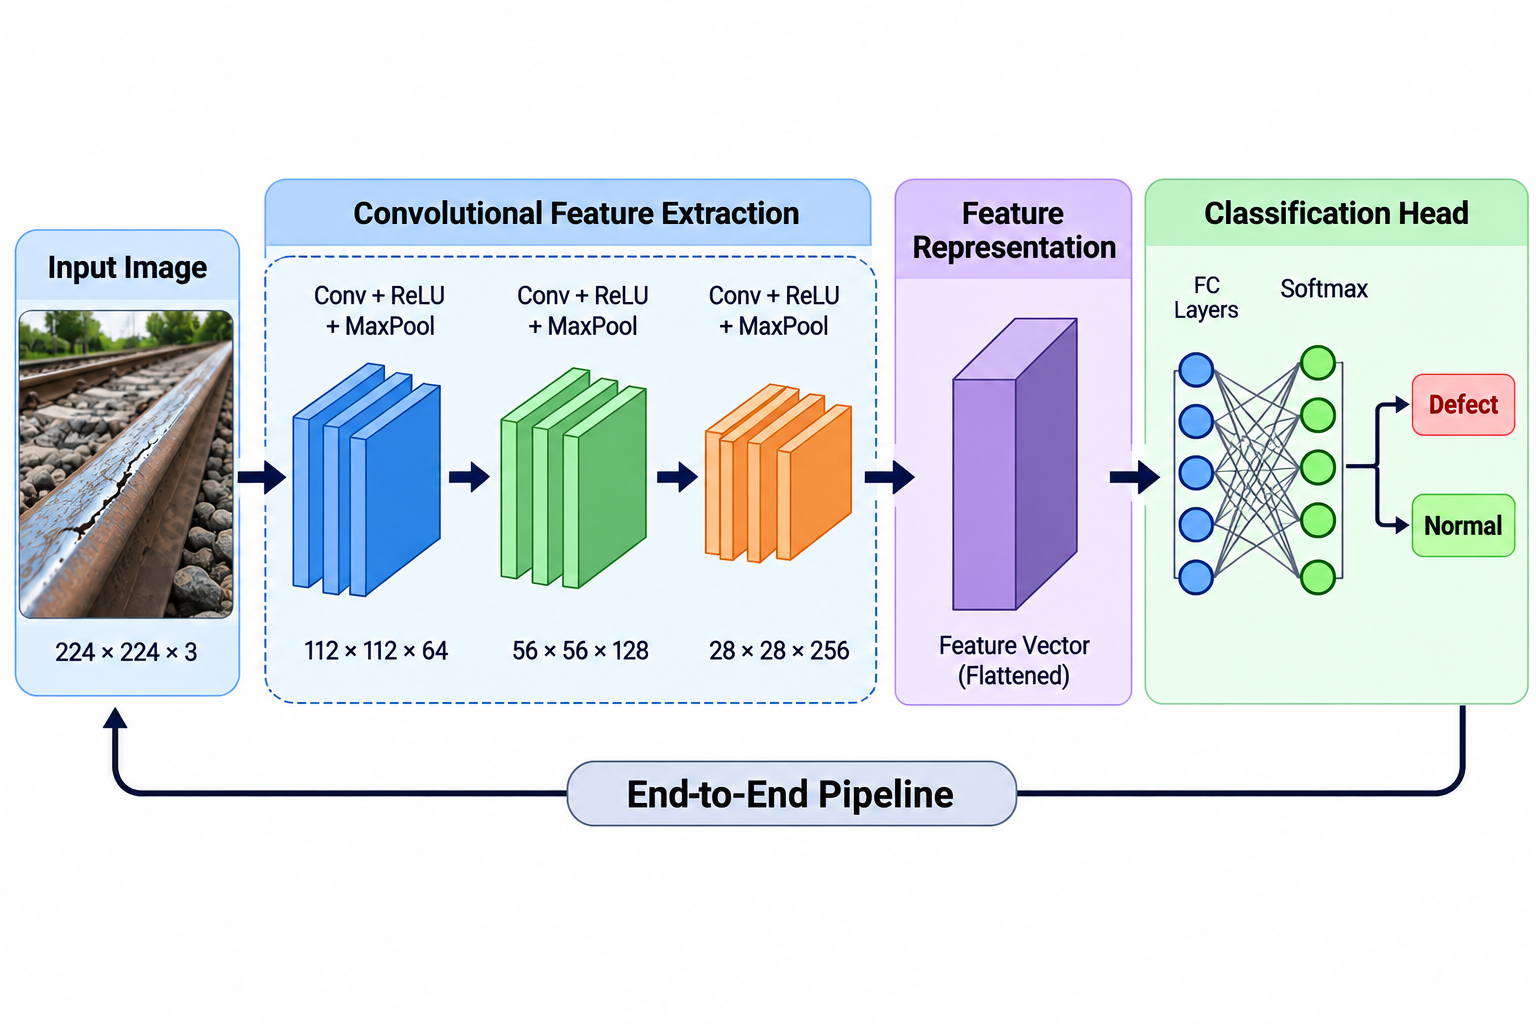
\includegraphics[width=\textwidth]{fig_architecture.png}
  \caption{CNN architecture for railway defect detection: Input image passes through four convolutional blocks with increasing filter depth (32, 64, 128, 256), global average pooling, a fully connected layer with dropout, and a binary output layer.}
  \label{fig:architecture}
\end{figure*}

The model was trained using the Adam optimiser with a learning rate of 0.001, categorical cross-entropy loss function, and data augmentation including random rotation ($\pm$15 degrees), horizontal flipping, and brightness adjustment to improve generalisation across environmental conditions. Training proceeded for 50 epochs with early stopping based on validation loss. The Adam optimiser was selected for its adaptive learning rate properties, which are particularly beneficial when training on datasets with noisy labels and variable feature distributions.

\subsection{Performance Results Under Ideal Conditions}

Table~\ref{tab:results} presents the classification performance metrics obtained under ideal laboratory conditions with the original dataset. The model achieves 93.2\% overall accuracy, with individual metrics indicating strong but imperfect defect detection capability.

\begin{table}[ht]
\caption{Model Performance Under Ideal Conditions}
\label{tab:results}
\centering
\renewcommand{\arraystretch}{1.2}
\begin{tabular}{|p{4.8cm}|c|}
\hline
\textbf{Metric} & \textbf{Value} \\
\hline
Overall Accuracy & 93.2\% \\
\hline
Precision & 94.1\% \\
\hline
Recall (Sensitivity) & 91.5\% \\
\hline
Specificity & 94.9\% \\
\hline
F1-Score & 92.8\% \\
\hline
\textbf{False Negative Rate (FNR)} & \textbf{8.5\%} \\
\hline
True Positives (TP) & 257 \\
\hline
False Positives (FP) & 16 \\
\hline
True Negatives (TN) & 283 \\
\hline
False Negatives (FN) & 24 \\
\hline
\end{tabular}
\end{table}

The false negative rate of 8.5\% warrants particular attention. This means that approximately 1 in 12 defective rail sections would be classified as normal by the model. In a safety-critical railway context where a single missed defect can cause a derailment, this rate is unacceptable without supplementary human review. The RDSO ultrasonic testing standard requires 100\% reliability in its testing context \cite{rdso2020}, establishing the high bar that any inspection system -- AI-assisted or otherwise -- must approach.

\subsection{Robustness Analysis Under Adverse Conditions}

We evaluated model performance under six environmental conditions to assess field-readiness. Figure~\ref{fig:robustness} presents the results. Performance degradation was systematically evaluated by applying image transformations simulating: (1) reduced illumination intensity, (2) additive Gaussian noise simulating surface contamination, (3) rust-coloured overlays simulating corrosion, (4) shadow patterns simulating vegetation occlusion, and (5) combined application of all adverse conditions.

\begin{figure}[ht]
  \centering
  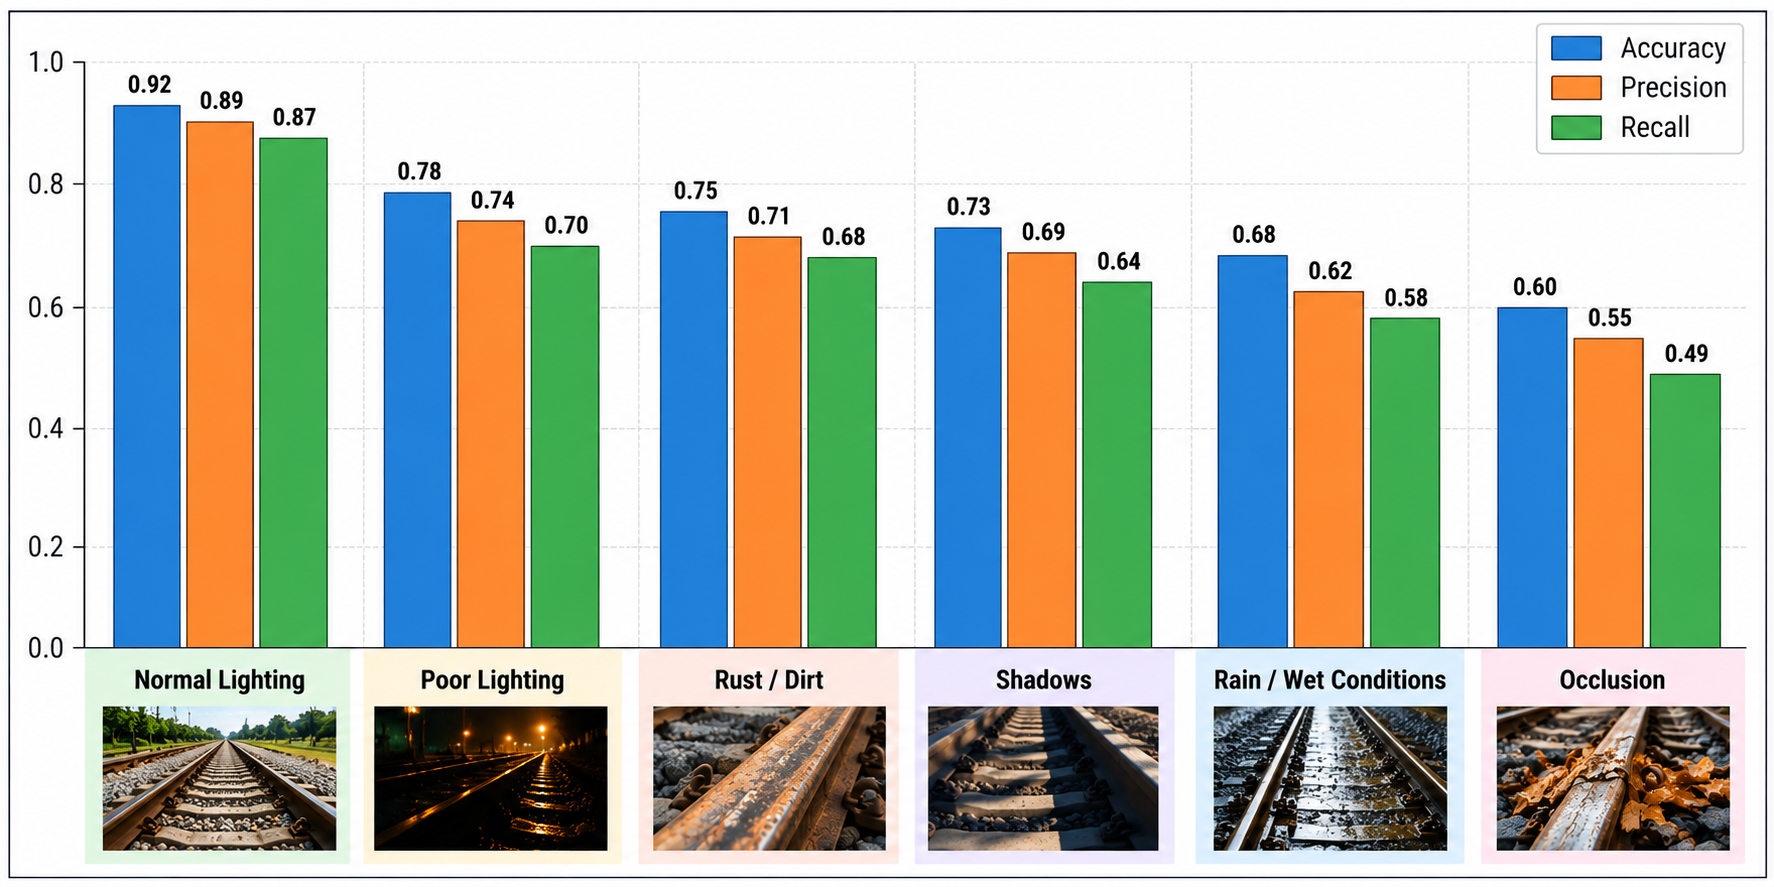
\includegraphics[width=\linewidth]{fig_robustness.png}
  \caption{Model performance under adverse environmental conditions. Accuracy (left) degrades from 93.2\% to 78.4\% under combined adverse conditions, while the False Negative Rate (right) -- the critical safety metric -- increases from 8.5\% to 22.7\%, a 2.7x deterioration.}
  \label{fig:robustness}
\end{figure}

The results reveal a disturbing pattern for safety-critical deployment. While accuracy drops from 93.2\% to 78.4\% under combined adverse conditions, the false negative rate escalates from 8.5\% to 22.7\% -- meaning that more than 1 in 4 defective rails would be missed under worst-case field conditions. This asymmetric degradation, where FNR increases much faster than overall accuracy declines, is characteristic of imbalanced datasets and underscores why accuracy alone is an insufficient safety metric. The 2.7x increase in FNR under adverse conditions represents the most significant finding of our experimental analysis: a model that appears safe in the laboratory may be dangerously unreliable in the field.

\subsection{Grad-CAM Explainability Results}

Figure~\ref{fig:gradcam} presents Grad-CAM visualisations for representative test cases across the three classification outcomes. Panel (a) shows a correctly detected crack where the heatmap accurately highlights the defect region, confirming that the model attended to the relevant surface feature. Panel (b) shows a missed defect where the heatmap reveals attention to the ballast region rather than the rail surface, indicating that the model learned spurious correlations from the training data. Panel (c) shows a false positive where the model attended to a shadow pattern resembling a crack morphology, illustrating how texture-based features can lead to incorrect classifications under challenging illumination.

\begin{figure}[ht]
  \centering
  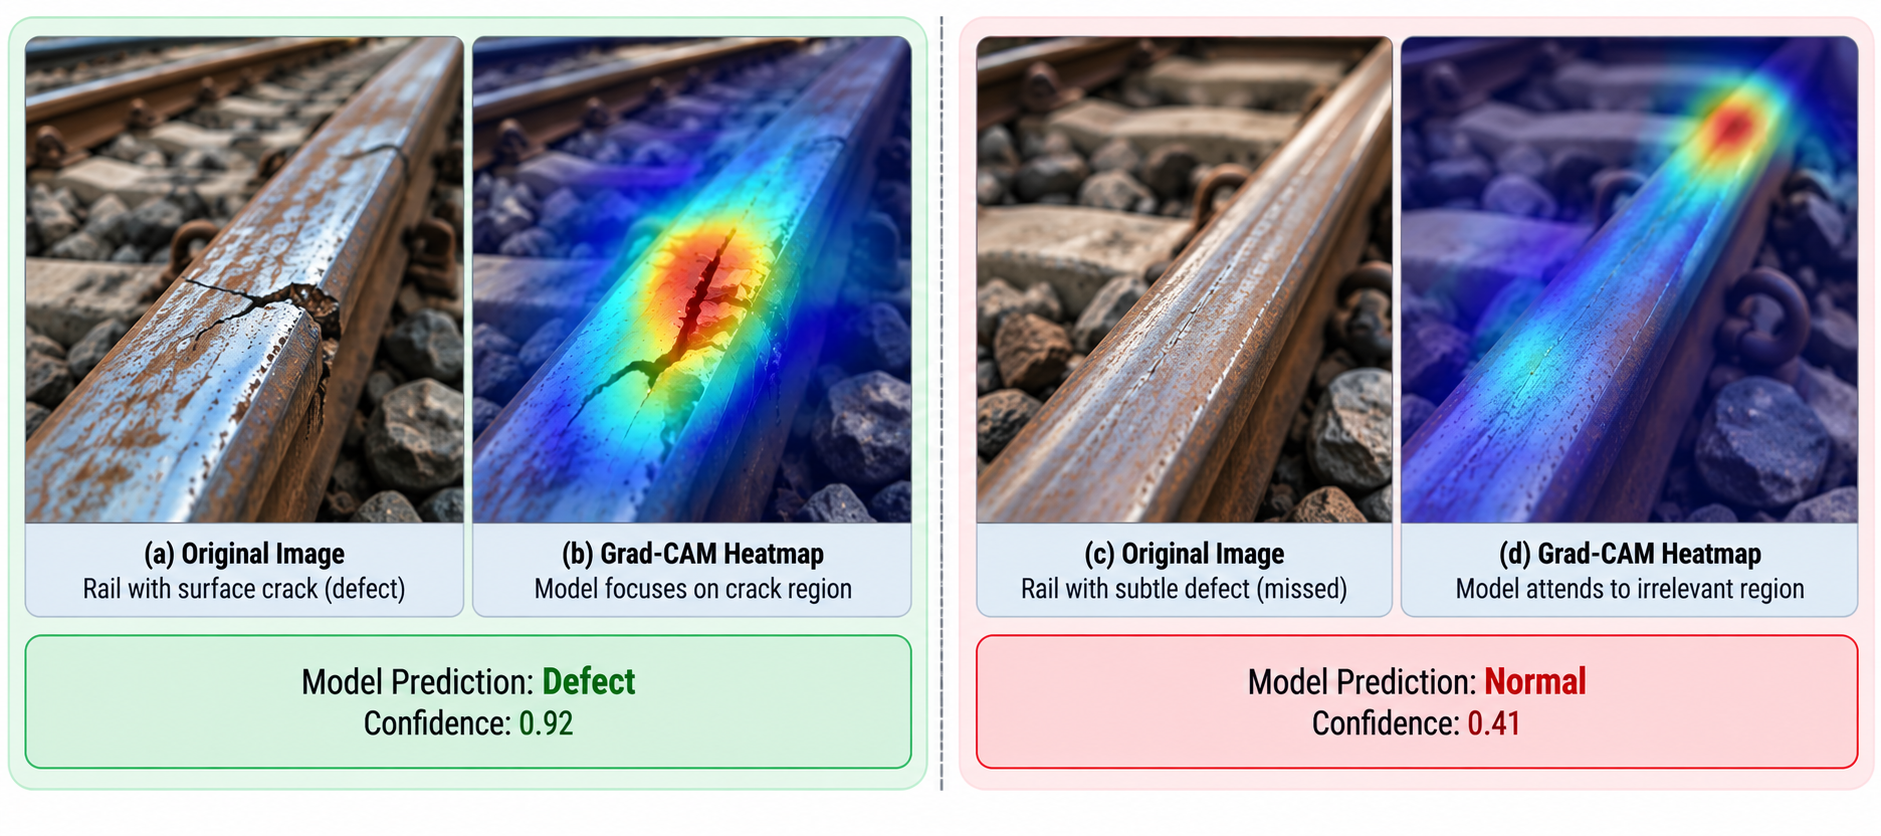
\includegraphics[width=\linewidth]{fig_gradcam.png}
  \caption{Grad-CAM explainability visualisations: (a) Correct detection with heatmap concentrated on crack region, (b) Missed detection with heatmap on irrelevant ballast region revealing spurious feature learning, (c) False positive with attention on shadow pattern mimicking crack morphology.}
  \label{fig:gradcam}
\end{figure}

These visualisations demonstrate that Grad-CAM provides actionable information for both model development -- identifying learned spurious features that degrade generalisation -- and operational deployment -- enabling inspector verification of AI reasoning before maintenance decisions are made.

% ============================================================
\section{Proposed Framework and Recommendations}
\label{sec:framework}
% ============================================================

\subsection{Human-in-the-Loop Framework}

Based on our analysis, we propose the human-in-the-loop framework illustrated in Figure~\ref{fig:framework}. The pipeline operates through seven stages designed to ensure that AI capabilities enhance rather than compromise railway safety:

\begin{figure*}[ht]
  \centering
  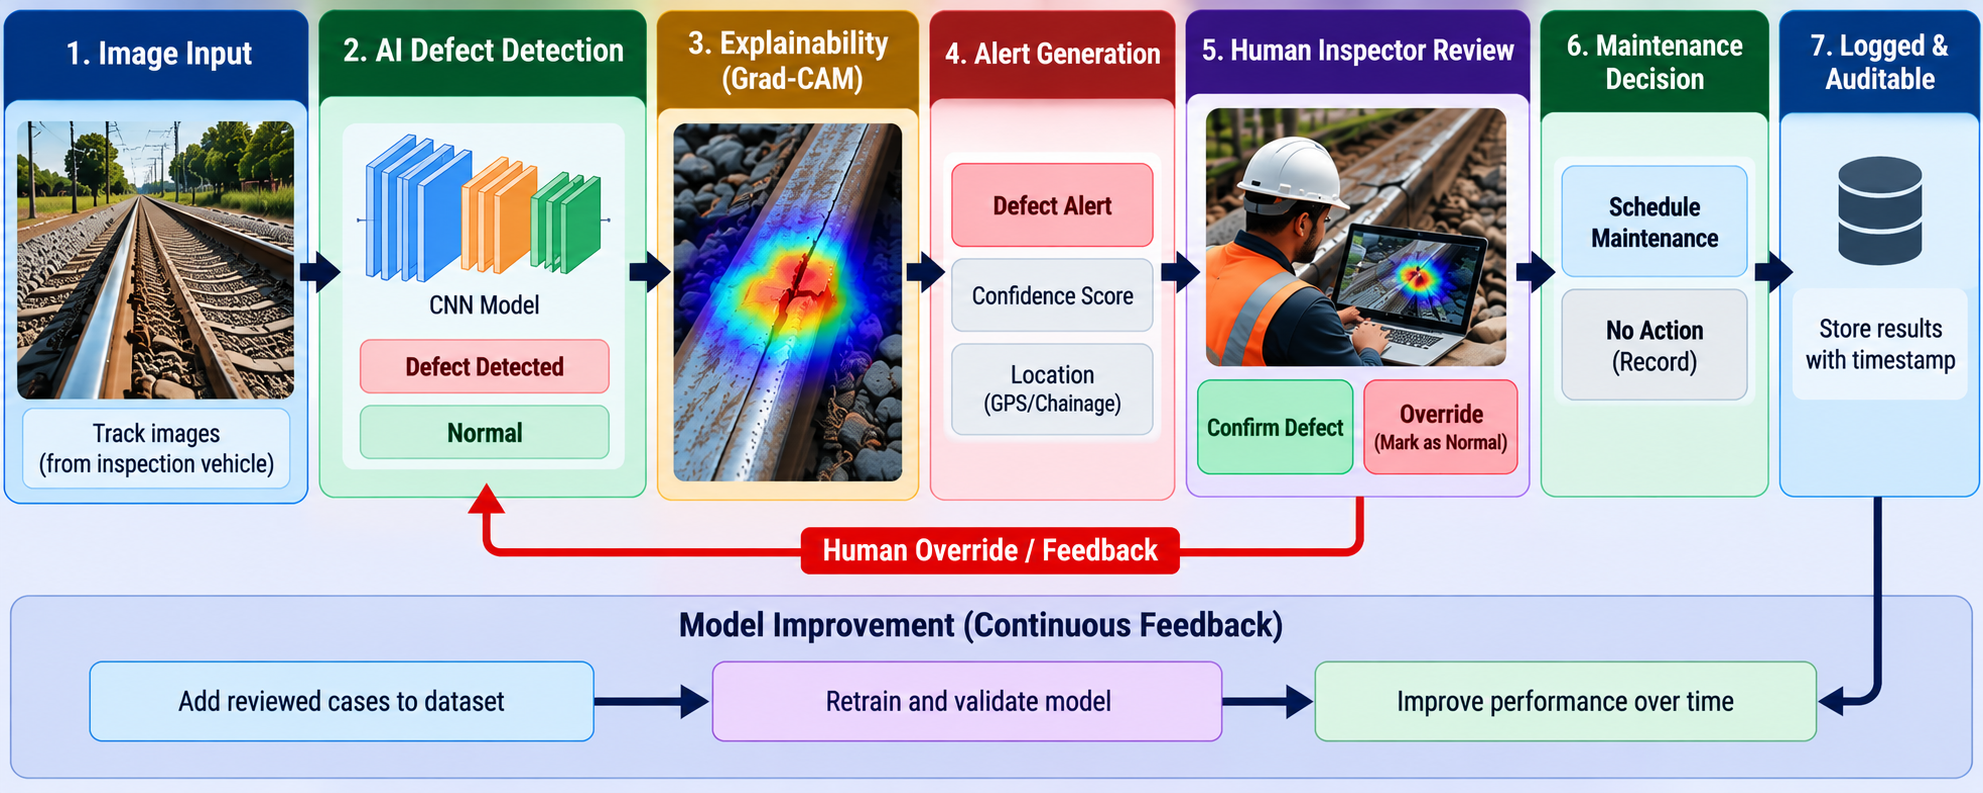
\includegraphics[width=\textwidth]{fig_framework.png}
  \caption{Proposed human-in-the-loop framework for AI-assisted railway track inspection, showing confidence-based routing, human inspector review with override capability, and auditable maintenance decisions aligned with RDSO procedures.}
  \label{fig:framework}
\end{figure*}

\begin{enumerate}
    \item \textbf{Image Acquisition:} High-resolution cameras mounted on inspection vehicles capture rail surface images at configurable intervals. Environmental metadata including lighting conditions, weather state, vehicle speed, and GPS location are recorded alongside each image for traceability and robustness analysis.
    \item \textbf{AI Pre-Screening:} The CNN model classifies each image as defective or normal, producing both a class label and a confidence score.
    \item \textbf{Explainability Layer:} Grad-CAM generates a heatmap highlighting the image regions that most influenced the classification decision.
    \item \textbf{Confidence-Based Routing:} The system applies tiered routing based on classification confidence:
    \begin{itemize}
        \item High confidence, defect classification $\rightarrow$ Flagged for qualified inspector review with Grad-CAM overlay.
        \item High confidence, normal classification $\rightarrow$ Logged for records and periodic audit sampling.
        \item Low confidence (below threshold) for any classification $\rightarrow$ Mandatory escalation for manual inspection per RDSO procedures.
    \end{itemize}
    \item \textbf{Human Inspector Review:} A qualified railway inspector reviews all flagged images alongside Grad-CAM visualisations, applies engineering judgement, and records a determination. The inspector retains unconditional authority to override the AI classification.
    \item \textbf{Maintenance Decision:} Based on inspector determination, maintenance is scheduled according to established RDSO procedures. Serious defects trigger immediate speed restrictions pending physical inspection.
    \item \textbf{Audit Trail:} All AI classifications, Grad-CAM visualisations, inspector determinations, and maintenance actions are logged in a tamper-evident record for regulatory compliance and continuous model improvement.
\end{enumerate}

The critical design principle is that the human inspector is not an afterthought but a mandatory checkpoint in the safety chain. The AI system pre-screens and prioritises, but the inspector decides.

\subsection{Key Recommendations}

Based on our investigation, we present seven recommendations for responsible AI deployment in railway track inspection:

\begin{enumerate}
    \item \textbf{Do not deploy as a standalone system.} AI-based visual inspection must operate as a decision-support tool within the existing railway inspection governance structure. RDSO ultrasonic testing procedures and qualified inspector judgement remain the authoritative safety layers.
    \item \textbf{Report false negative rate as the primary safety metric.} Overall accuracy is insufficient for safety-critical evaluation. Always report FNR alongside precision, recall, and F1-score, and evaluate FNR separately under each environmental condition.
    \item \textbf{Maintain ultrasonic testing requirements.} Visual AI inspection cannot replace non-destructive testing for internal rail flaws. The proposed system augments existing procedures, not replaces them.
    \item \textbf{Implement confidence-based escalation.} Low-confidence classifications must trigger mandatory human review. Automatic acceptance or rejection of uncertain predictions creates unacceptable safety risk.
    \item \textbf{Establish explicit accountability chains.} Define who reviews AI alerts, who authorises maintenance, and who bears responsibility for safety decisions. These roles must be documented and aligned with existing Indian Railways organisational structure.
    \item \textbf{Conduct environmental robustness testing.} Validate model performance across the full range of conditions specific to each railway division before deployment. Retrain or recalibrate models for regional conditions.
    \item \textbf{Include explainability from the design phase.} Grad-CAM and similar tools should be integral to the system architecture, not retrofitted for compliance. Inspectors trained on the system should understand how explanations are generated and their limitations.
\end{enumerate}

% ============================================================
\section{Conclusion}
\label{sec:conclusion}
% ============================================================

AI-based railway track defect detection offers significant potential to enhance the safety and efficiency of Indian railway infrastructure. However, this potential can only be realised through responsible deployment that respects the safety-critical nature of the domain. Our investigation yields five key findings:

First, \textbf{high accuracy does not guarantee safety}. A model achieving 93\% accuracy under ideal conditions still misses approximately one in twelve defects, and up to one in four under adverse field conditions. The false negative rate, not overall accuracy, is the critical safety metric.

Second, \textbf{explainability is essential but insufficient}. Grad-CAM visualisations help inspectors verify AI reasoning and help developers identify model weaknesses, but they do not prove that a classification is correct. Explainability builds trust and aids debugging; it does not replace independent verification.

Third, \textbf{human oversight must be preserved}. AI should augment, not replace, qualified railway inspection. The inspector's ability to override AI classifications, escalate uncertain results, and apply engineering judgement is a safety requirement, not a governance inconvenience.

Fourth, \textbf{accountability must be explicit}. The governance framework must clearly define roles for alert review, maintenance authorisation, and safety responsibility, aligned with existing Indian Railways organisational structures and RDSO technical standards.

Fifth, \textbf{AI supports existing procedures}. Visual inspection using cameras and AI augments the railway inspection toolkit. It cannot and should not replace ultrasonic testing, patrolling, or the professional judgement of qualified railway engineers.

Future research directions include: collecting representative datasets from multiple Indian railway divisions with diverse environmental conditions; developing multi-sensor fusion architectures combining visual, acoustic, and ultrasonic data; establishing regulatory standards and certification frameworks for AI-assisted railway inspection systems; and conducting longitudinal studies of AI-assisted inspection outcomes to measure safety improvements over traditional methods alone.

The responsible deployment of AI in railway inspection is not merely a technical challenge -- it is a safety and governance imperative. The lives of millions of daily passengers depend upon the integrity of the tracks they travel upon, and that integrity must be assured by systems that are reliable, explainable, accountable, and firmly grounded in established railway safety practice.

% ============================================================
\section*{Acknowledgments}
% ============================================================
The authors acknowledge the use of publicly available datasets and open-source tools for this research. We thank the Research Designs and Standards Organisation (RDSO) for publicly available inspection standards that informed our analysis, and the Ministry of Railways for documentation of existing inspection technologies.

% ============================================================
\bibliographystyle{IEEE}

\begin{thebibliography}{16}

\bibitem{pib2017}
Press Information Bureau, Government of India, ``Hi-Tech System To Detect Railway Track Defects,'' Dec. 15, 2017. [Online]. Available: \url{https://www.pib.gov.in/PressReleaseIframePage.aspx?PRID=1512776}

\bibitem{rdso2020}
Research Designs and Standards Organisation (RDSO), \textit{Indian Railway Standard Specification for Ultrasonic Testing of Rails/Welds}, Document No. T-53, Revised 2020.

\bibitem{ieee2025}
``Recent Advances and Innovative Approaches to Railway Safety Based on Applications, Sensors and Algorithms: A Systematic Review,'' \textit{IEEE Access}, vol. 13, pp. 200271--200289, 2025, doi: 10.1109/ACCESS.2025.3634804

\bibitem{khajeh2025}
A. Khajehdezfuly, H. Azizipour, and S. Kaewunruen, ``A review of applications of AI in monitoring, inspection, and maintenance of railway tracks,'' \textit{Journal of Industrial Information Integration}, vol. 48, Art. no. 101005, 2025, doi: 10.1016/j.jii.2025.101005

\bibitem{alif2026}
M. A. R. Alif, G. Tucker, and M. Hussain, ``Advances in computer vision for comprehensive railway engineering: from track inspection to rolling stock and safety monitoring,'' \textit{Railway Engineering Science}, 2026, doi: 10.1007/s40534-026-00434-7

\bibitem{yolo2024}
``Automated Railway Crack Detection Using Machine Learning: Analysis of Deep Learning Approaches,'' in \textit{Proc. IEEE 15th Annual Information Technology, Electronics and Mobile Communication Conference (IEMCON)}, 2024, doi: 10.1109/IEMCON62851.2024.11093324

\bibitem{kumar2025}
A. Kumar and S. P. Harsha, ``A systematic literature review of defect detection in railways using machine vision-based inspection methods,'' \textit{International Journal of Transportation Science and Technology}, vol. 18, pp. 207--226, 2025, doi: 10.1016/j.ijtst.2024.06.006

\bibitem{zenodo2023}
``Railways -- Rail Track Surface Fault \& Defect Detection Based on Deep Learning,'' \textit{Zenodo}, 2023. [Online]. Available: \url{https://zenodo.org/}

\bibitem{selvaraju2017}
R. R. Selvaraju, M. Cogswell, A. Das, R. Vedantam, D. Parikh, and D. Batra, ``Grad-CAM: Visual Explanations from Deep Networks via Gradient-Based Localization,'' in \textit{Proc. IEEE ICCV}, 2017, pp. 618--626.

\bibitem{wang2022}
W. Wang, C. Zhu, L. Zhang, and Y. Zhang, ``Detection of Surface Defects on Railway Tracks Based on Deep Learning,'' \textit{IEEE Access}, vol. 10, pp. 126451--126465, 2022, doi: 10.1109/ACCESS.2022.3224594

\bibitem{northernrail2021}
Northern Railway, \textit{Indian Railways Unified Standard Schedule of Rates}, 2021, Chapter 14: Testing of Rails and Other Components.

\bibitem{hspr2026}
``Multi-class rail defect detection using advanced artificial intelligence,'' \textit{Health and Social Care in the Community}, 2026, doi: 10.1016/j.hspr.2026.03.002

\bibitem{zhang2019}
``Review of Applications of Visual Inspection Technology Based on Image Processing in the Railway Industry,'' \textit{Transportation Safety and Environment}, vol. 1, no. 3, pp. 185--204, 2019, doi: 10.1093/tse/tdz007

\bibitem{he2016}
K. He, X. Zhang, S. Ren, and J. Sun, ``Deep Residual Learning for Image Recognition,'' in \textit{Proc. IEEE CVPR}, 2016, pp. 770--778.

\bibitem{tan2019}
M. Tan and Q. Le, ``EfficientNet: Rethinking Model Scaling for Convolutional Neural Networks,'' in \textit{Proc. ICML}, 2019, pp. 6105--6114.

\bibitem{fumera2002}
G. Fumera, F. Roli, and G. Giacinto, ``Reject option with multiple thresholds,'' \textit{Pattern Recognition}, vol. 33, no. 12, pp. 2099--2101, 2002.

\end{thebibliography}

\end{document}
